\documentclass[11pt,a4paper]{article}
\usepackage{fontspec}
\setmainfont{Source Serif 4}[Path=/home/claude/ref/fonts/, UprightFont=SourceSerif4-Regular.ttf, BoldFont=SourceSerif4-Semibold.ttf, ItalicFont=SourceSerif4-It.ttf]
\setmonofont{IBM Plex Mono}[Path=/home/claude/ref/fonts/, UprightFont=IBMPlexMono-Regular.ttf, BoldFont=IBMPlexMono-Medium.ttf, Scale=0.88]
\usepackage[a4paper,margin=2.4cm]{geometry}
\usepackage{amsmath}
\usepackage{graphicx,booktabs,float,caption,array,xcolor,longtable}
\usepackage{xurl}
\usepackage[hidelinks]{hyperref}
\usepackage[round]{natbib}
\usepackage{setspace}
\setstretch{1.08}
\renewcommand{\topfraction}{0.9}
\renewcommand{\bottomfraction}{0.8}
\renewcommand{\textfraction}{0.1}
\renewcommand{\floatpagefraction}{0.75}
\setlength{\parindent}{0pt}
\setlength{\parskip}{0.55em}
\captionsetup{font=small,labelfont=bf}
\setlength{\bibsep}{3pt}
\urlstyle{same}
\hypersetup{pdftitle={A Day from London},pdfauthor={Dr Tristan Hotham}}

\begin{document}
\begin{center}
{\Large\bfseries A Day from London: One-Day Travel Reach across Great Britain in 1750, the 1830s, 1850, 1910 and Today, from a Calibrated Historical Network Model\par}
\vspace{1.2em}
{\large Dr Tristan Hotham\par}
\vspace{0.3em}
{\small Independent researcher\\
ORCID: 0000-0003-4931-9349\\
DOI: https://doi.org/10.5281/zenodo.24105505\par}
\vspace{0.8em}
2026
\end{center}

\begin{quote}
\small
\begin{center}\textbf{Abstract}\end{center}
How much of Great Britain lay within a day's travel of London, and how did that change between the coaching era and today? I build a multimodal network model on a 2 km grid for five dates (1750, the 1830s, 1850, 1910 and today) from historical GIS of the turnpike roads of England and Wales and the railways of 1851, a reconstruction of the 1910 rail network, and OpenStreetMap. Coach speeds are fitted to scheduled times of London coach services in 1836 (136 destinations) and to twelve cited journeys of 1739 to 1764; train speeds come from published averages; every era is tested on journeys it was not fitted to. The 1830s model reproduces the 1837 mail-coach timetable with a median absolute error of 12\%. The 1750 model fails the error threshold set in advance (28\% against 25\%), so its map is a rough sketch. The 1850 and 1910 models use average train speeds and are slower than documented expresses by a median 46\% and 34\%, on four and six journeys, so their areas are lower bounds. Leaving Charing Cross at dawn, twelve hours of travel reached 5\% of Great Britain's land in 1750, 19\% in the 1830s, at least 47\% in 1850, at least 72\% in 1910 and 97\% today. The largest gain per year came between the 1830s and 1850, when the first railways multiplied the area within a day by at least 2.5 in about fifteen years. The surfaces and code are released for reuse.

\textbf{Keywords:} time-space convergence; accessibility; turnpike roads; stagecoaches; railways; historical GIS; Great Britain
\end{quote}

\section{Introduction}
In 1754 a coach advertised that it would carry passengers from London to Edinburgh in ten days in summer and twelve in winter \citep{harper1922}. In 1837 the Edinburgh mail coach was timed at 42 hours and 23 minutes \citep{harper1903}. By the early 1900s the Flying Scotsman ran from King's Cross to Edinburgh in eight hours and a quarter \citep{wiki_fs}, and today the fastest train is timed at four hours \citep{visitlondon}. These are the familiar milestones of the transport revolution, and they have been told many times as falling journey times between pairs of famous places. What they do not show is the whole map: how much of the country lay within a day of the capital, and where the edge of that day fell, in each era.

This paper draws that map. It asks a simple question: leaving Charing Cross at dawn, how much of Great Britain could a traveller reach within twelve hours of travel in 1750, in the 1830s, in 1850, in 1910 and today? To answer it I build a transparent multimodal network model on a 2 km grid. Its road layer for 1750 and the 1830s is the turnpike and main road map of England and Wales digitised by \citet{rosevear2023tp}, with each section coded by whether it was a turnpike in that decade; its coach speeds are calibrated, one parameter per era, on documented journey times, including 136 London destinations with scheduled times in 1836 \citep{bates1969,rosevear2023coach}. Its rail layer for 1850 is the 1851 network digitised by the Cambridge Group \citep{satchell2023}, for 1910 a reconstruction from that network, today's lines and the stations that closed after 1910, and today's network from OpenStreetMap. Train speeds come from Leunig's (\citeyear{leunig2006}) estimates of average speeds on English and Welsh railways, and everything is checked against documented journeys that were not used to set the speeds.

The answer is a sequence of five maps (Figure~\ref{fig:maps}). In 1750 a day's coaching from London covered 11,144 km$^2$, 5\% of Great Britain's land, a patch reaching roughly 66 km from Charing Cross. On the faster coaches and better roads of the 1830s it covered 19\%. The railway of 1850 pushed the edge of the day to 47\%, the network of 1910 to 72\%, and today 97\% of the land can be reached within twelve hours by car or train. These numbers are not equally firm. The 1750 model misses its documented journeys by more than the limit set in advance, so the 1750 map is a rough sketch; the railway models use average trains and are much slower than the documented expresses, so the 1850 and 1910 areas are lower bounds (Section~\ref{sec:results}). Between 1750 and today the area within a day of London grew 20-fold. The most rapid shrinking of the country happened twice: between 1750 and the 1830s, on the roads, and between the 1830s and 1850, when the first railways more than doubled the day's reach in about fifteen years.

The paper makes three contributions. First, it turns the well known point-to-point story of time-space convergence \citep{janelle1968,janelle1969} into a continuous, national surface for five dates, built from published historical GIS of roads and railways rather than from straight lines or a handful of routes. Second, it calibrates and tests that surface openly: every speed is either fitted to cited timetables or taken from a published estimate, and every era's model is compared with journeys it was not fitted to, so readers can see how far to trust each map. The 1830s model, fitted on the 1836 coach timetables, reproduces the 1837 mail-coach timetable to within 12\% (median absolute error); the 1750 model, built on a dozen cited journeys, fails the error threshold set in advance and is a rough sketch; and the railway models, checked against only four and six documented express journeys, are much slower than those expresses, so their areas are lower bounds. Third, the derived grids, isochrones and the compiled journey times are released for reuse.

Section~\ref{sec:lit} reviews the literature on time-space convergence, pre-railway road transport and railway speeds. Section~\ref{sec:data} describes the data, Section~\ref{sec:model} the model, its calibration and the analysis plan, Section~\ref{sec:results} the results, Section~\ref{sec:robust} the checks, and Section~\ref{sec:disc} the limitations.

\section{Background and literature}\label{sec:lit}
\subsection{Time-space convergence and accessibility}
Janelle introduced the idea of time-space convergence: as transport improves, the travel time between places falls, so that in time, if not in space, places move closer together \citep{janelle1968}. He measured it as the average rate at which travel time between a pair of places falls, in minutes per year, and linked it to the reorganisation of activities around the places that gain most \citep{janelle1969}. The concept has since been carried into time-space maps, which redraw a territory so that distances on the page are proportional to travel times \citep{spiekermann1994}, and into long-run measures of accessibility, such as the Swiss reconstruction since 1850 by \citet{axhausen2011}, which found road accessibility overtaking rail around 1930. Cultural histories describe the same change as a ``shrinking'' of space and an industrialisation of time \citep{schivelbusch1986}. Historical work on London itself shows how rail access and population density developed together \citep{levinson2008}. These studies share a need for travel times that are comparable across eras and across space. The present paper supplies them for Britain from a single model applied to five network states.

\subsection{Roads and coaches before the railway}
The literature on the turnpike era is rich in quantitative evidence. Turnpike trusts, local bodies empowered by Acts of Parliament to levy tolls and improve a stretch of road, are the subject of classic studies \citep{albert1972,pawson1977}; by 1838, on the map used here, nearly 23,000 miles of road were under active turnpike trusts \citep{rosevear2023tp}. Historical atlases map coach journey times from London around 1750 and in the 1830s \citep{pope1989}. \citet{bogart2005} assembled journey times from the coaching literature and showed that average passenger journey speeds rose from 2.6 miles per hour in the 1750s to 8.0 in the 1820s, measuring distance over total elapsed journey time, and linked the gains to turnpike investment: the London to Birmingham journey fell from 65 hours in 1705 to 40 hours in 1740 and 25 hours in 1770 as trusts took over the route. \citet{gerhold2014}, using newspaper advertisements from 1653 to 1840, dated the acceleration of London coaches to two periods, the 1760s to 1780s and the 1810s to 1820s, and attributed it to turnpikes, better vehicles and better horses. \citet{gerhold2005} documents the carriers and coaches of the pre-turnpike era.

The Cambridge Group's transport project has turned this evidence into historical GIS. The turnpike map used here records every turnpike and main road of England and Wales from about 1680 to 1850, built from Cary's maps and the Acts, with the decade in which each section was a turnpike \citep{rosevear2023tp}. A companion file maps the routes and scheduled times of London coach services in 1819 (from Cary's \textit{New Itinerary}) and 1836 \citep{bates1969,rosevear2023coach}. These data have been used to study the geography of coaching \citep{rosevear2018} and, with assumed average speeds per mode, to estimate transport costs and their fall between 1680 and 1830 \citep{alvarez2017}, who assume 2 miles per hour for passengers by road in 1680 and 8.7 mph in 1830 (the average for journeys of 80 miles and more in Gerhold's sample). The present paper uses the same road map but fits the speed to scheduled times rather than assuming it, and extends the comparison to the railway era and today.

Older narrative sources record many individual journeys. Smiles's history of roads and travelling \citep{smiles1867} and Harper's road books \citep{harper1899,harper1902,harper1903,harper1922} quote advertisements, diaries and time-bills. Jackman's survey remains the fullest general account \citep{jackman1916}. These sources are uneven and sometimes repeat each other, and a stated duration in days leaves the hours on the road unknown. They are used here for what they are: a set of documented journeys, each cited, against which a model can be checked.

\subsection{Railway speeds}
The railway network of England, Wales and Scotland has been reconstructed as a time-dynamic GIS from Cobb's atlas by the Cambridge Group and the University of Lleida, with snapshots for 1851, 1861 and 1881 released publicly \citep{marti2017,satchell2023}. It has been used to measure how quickly railways reached the population and whether stations brought growth \citep{gregory2010,bogart2022}, and set in a European context \citep{marti2013}. For speeds, \citet{leunig2006} transcribed timetables for important and minor routes in England and Wales in 1850, 1870, 1887 and 1910 and estimated average in-train speeds, measured on a straight-line basis, of 22.7 mph on important journeys and 17.8 mph on minor ones in 1850, rising to 36.9 and 20.4 mph in 1910 \citep[Table~2]{leunig2006}. Those averages are the train speeds of this model.

\subsection{Contribution}
What is missing is a single, testable surface of travel time across the whole of Great Britain that can be compared across the coach and rail eras. Point-to-point histories cannot say how much of the country lay within a day of London; maps such as Pawson's give isochrones for coach journeys but not a common method that carries through the railway age; and economic studies that build network models usually assume speeds rather than test them against timetables. This paper builds one model, calibrates one speed per era where data allow, takes published speeds where they do not, and reports how well each era's map reproduces journeys it has not seen.

\section{Data}\label{sec:data}
\subsection{Roads, 1750 and the 1830s}
The road layer for England and Wales is the ``turnpikes and main'' shapefile of \citet{rosevear2023tp}: 23,556 features (23,756 line parts once multi-part features are split) and about 41,000 miles of road, including every turnpike, the ``other main roads'' of Cary's maps, link roads, bridges and ferries. For each decade from 1750 to 1850 a field records whether the section was a turnpike at that date; roads that were not yet built (new alignments) are coded separately and dropped from earlier networks. In the 1750 network a section is either a turnpike in 1750 or an existing main road that was not; the same for 1830 (and 1820 for the 1819 check, 1838 for the feeder roads of 1850 and 1910). The map does not cover Scotland. For Scotland I use today's trunk and primary roads from OpenStreetMap as a proxy for its main roads, at the non-turnpike speed in 1750 and the turnpike speed in the 1830s. This matters only for the far north, which lies well beyond a day from London in both coach eras.

\subsection{Coach timetables, 1819 and 1836}
The London coaches file \citep{rosevear2023coach} maps 640 timed coach routes that start in London, each drawn on the turnpike map, with scheduled journey times where the source gives one. Leaving out short stages whose terminus is less than 15 km from Charing Cross, 283 timed services in 1836 reach 136 distinct termini, and 357 services in 1819 reach 147. The median scheduled speed of all timed 1836 services, measured along the mapped route, is 8.2 mph, and 9.0 mph for routes of 80 miles or more, close to the 8.7 mph that \citet{alvarez2017} take from Gerhold. For calibration I keep the fastest service to each terminus, because the question is how far a traveller could get, and take the far end of the route as the terminus point.

\subsection{Railways, 1850 and 1910}
The 1850 rail layer is the 1851 England, Wales and Scotland rail lines snapshot \citep{satchell2023}: 1,431 polylines, 6,336 miles of line open for passengers or freight during 1851 (the file does not distinguish the two). There is no public snapshot for 1910: the full time-dynamic file is restricted to the project teams \citep{marti2017}. I therefore reconstruct the 1910 network from three parts: the 1851 lines (nearly all still open in 1910); today's railway lines from OpenStreetMap; and lines that have since closed, inferred from the 2,167 stations in a list of closed British stations that closed after 1910 and lie more than 2 km from either of the first two sets. These stations are joined by a minimum spanning tree with links of at most 15 km, and each group to the nearest line, adding 8,827 km of inferred line. The inferred lines are straight segments between stations, so their lengths are too short where real lines curved, and a few will join stations that were never connected. Lines opened after 1910 and still open (the Channel Tunnel Rail Link, for example) are not removed. Rail sections are classed as main lines when at least half their length lies within 250 m of a line that OpenStreetMap shows at zoom level 8 (a proxy for today's main lines) and as branch lines otherwise.

Stations determine where a traveller can board. In 1850 they are the open stations whose Wikidata opening year is 1850 or earlier, plus closed stations within 500 m of an 1851 line; in 1910, open stations opened by 1910 plus every station closed after 1910; today, the stations open today. A rail vertex within 1.5 km of a station can be boarded.

\subsection{Today}
Today's road layer is the OpenStreetMap network of motorways, trunk, primary and secondary roads, read from OpenFreeMap vector tiles at zoom level 10 (OSM positional accuracy is high on main roads; \citealp{haklay2010}). Today's rail layer is the OpenStreetMap railway network (standard gauge lines, not sidings, trams or the Underground), with today's open stations.

\subsection{Documented journeys}
For each era I compiled documented journey times from London with a source for each (Appendix Table~\ref{tab:docs}). For 1750, the twelve journeys between 1739 and 1764 that I could find and cite, to nine towns: from \citet{smiles1867}, \citet{bogart2005}, Harper's road books and a summary of Gerhold's York services of 1764 \citep{gnrsite}. Journeys given in days are converted at twelve travelling hours a day, which is also the length of the day modelled; the sensitivity to ten and fourteen hours is reported. The thirty to sixty journeys per era that a firm calibration would want could not be found in sources reachable for this study, and this is the weakest part of the evidence. For the 1830s, the 1836 timetables above for calibration and, as an out-of-sample test, the list of 27 mail coaches leaving London nightly in 1837 printed by \citet{harper1903}. For the railway eras, the fastest documented times I could cite: to Liverpool in 1851 \citep{sidney1851}, Aberdeen in 1855 \citep{wiki_race}, Edinburgh in 1862 \citep{wiki_fs} and Birmingham on the first timetable of 1838 \citep{tring} for 1850; Edinburgh, Glasgow, Plymouth, Penzance, Bristol and Aberdeen between 1896 and 1904 for 1910 \citep{wiki_fs,harper1903,wiki_cre,wiki_cornishman,wiki_race}; and the fastest times from London to twelve cities stated by \citet{visitlondon} for today.

\section{Model and design}\label{sec:model}
\subsection{Graph}
Great Britain is divided into 2 km cells on the British National Grid; a cell is land if its centre lies inside a local authority of England, Wales or Scotland, giving 57,524 cells and 230,096 km$^2$. Each era's graph has three kinds of edge. Walking edges join each land cell to its eight neighbours at 4.8 km/h (3 mph); today these edges stand for minor roads at 30 km/h. Network edges follow each road or rail line, resampled every 300 m, at the speed of that line; vertices of different lines within 40 m of each other are joined, which connects junctions and the seams of the vector tiles. Access edges join each network vertex to the cell that holds it, at walking speed for the distance between them, with a wait of 30 minutes on boarding a train (and, in 1850 and 1910, a feeder coach); alighting is free. Ferries in the turnpike map carry a 30 minute wait. Travel times from the cell holding Charing Cross are found with Dijkstra's algorithm \citep{dijkstra1959}; the time to a town is the smallest time to any node within 2.5 km plus the walk from that node. The model has no timetables: it assumes a service is there when the traveller is, beyond the fixed waits.

\subsection{Speeds and calibration}
In the coach eras the free parameter is the speed of a coach on a turnpike, $v_T$, with existing main roads that were not turnpikes at $r = 0.6$ of that speed (a stated assumption, varied from 0.4 to 1.0). For the 1830s, $v_T$ is chosen on a grid of 0.5 km/h steps to minimise the sum of squared log errors between modelled and scheduled times for the fastest 1836 service to each of the 136 termini; for 1750, on a grid of 0.25 km/h steps against the twelve cited journeys. The same fit on the 1819 times, using the turnpikes of 1820, checks that the fitted speeds follow the trajectory in the literature. In 1850 and 1910 feeder coaches run on the 1838 turnpike network at the 1830s speeds.

Train speeds in 1850 and 1910 come from \citet[Table~2]{leunig2006}. His averages are in-train speeds measured along the straight line between the ends of a journey; I convert them to speeds along the track by multiplying by the median circuity of each era's rail network (network distance over straight-line distance) from Charing Cross to the 30 largest towns of England and Wales on the town list that lie within 5 km of each network (23 in 1850, all 30 in 1910): 1.15 in 1850 and 1.05 in 1910. Main lines run at Leunig's important-journey speed, 42.1 km/h in 1850 and 62.6 km/h in 1910, and branch lines at the ratio of his minor to important speeds (0.78 and 0.55). These speeds describe an average train, not the fastest express. Today's main-line speed is fitted, as in the coach eras, to the twelve fastest times from London, with branch lines at half that speed; today's road speeds are fixed at 100 km/h on motorways, 80 on trunk roads, 60 on primary and 45 on secondary roads, below the 2024 average free-flow car speeds of 68 mph on motorways and 51 mph on rural single carriageways \citep{dft2025} to allow for junctions, towns and traffic. A traveller today takes whichever of car or train is faster.

\subsection{Analysis plan}
The analysis was pre-specified in a written plan, kept in the study notes, before any travel time was computed: the twelve-hour day, the 2 km grid, the graph and its fixed parameters, one fitted speed per era, leave-one-destination-out validation, the out-of-sample tests, the headline outputs and the sensitivity checks below. One change was made before any calibration or validation was run, and is recorded in the notes: too few documented railway times could be found to fit train speeds for 1850 and 1910, so those come from Leunig's published averages, with a fit to the documented fastest trains kept as a sensitivity check. The plan named in advance what would count against the model: a leave-one-out median absolute error above 25\% in an era, or a mean log error beyond $\pm0.1$.

\subsection{Validation and uncertainty}
For the fitted eras, validation is leave one destination out: the speed is refitted without the destination and its time predicted. I report the number of journeys, the median absolute percentage error (MdAPE), the share within 20\% and the mean log error (bias). For 1850 and 1910 every documented journey is out of sample. On the maps the uncertainty of each era is shown by redrawing the twelve-hour line with all speeds raised and lowered by that era's median absolute error.

\section{Results}\label{sec:results}
\begin{figure}[tbp]\centering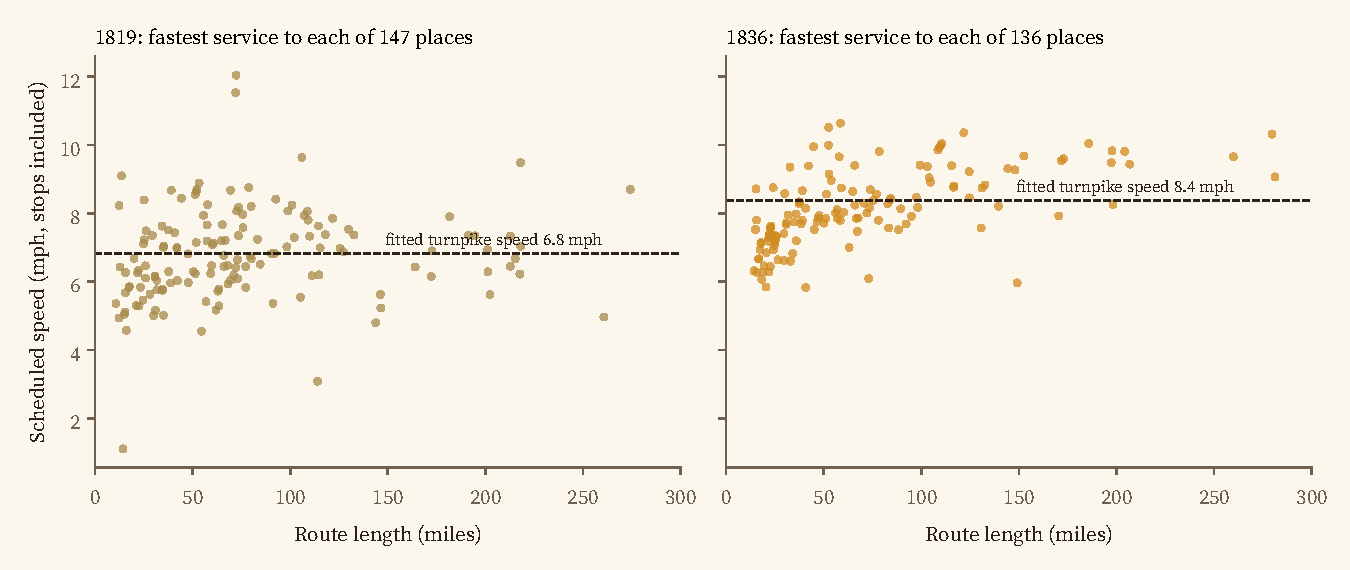
\includegraphics[width=0.95\textwidth]{f_coach.pdf}\caption{Scheduled speeds of the fastest London coach to each terminus, 1819 and 1836, against route length, with the fitted turnpike speed.}\label{fig:coach}\end{figure}
\subsection{Calibrated speeds}
Table~\ref{tab:speeds} lists every speed in the model and Figure~\ref{fig:coach} shows the coach timetables. Fitted to the fastest scheduled service to each of 136 termini in 1836, the turnpike coach speed is 13.5 km/h (8.4 mph), with non-turnpike main roads at 8.1 km/h. Fitted in the same way to 147 termini in 1819, on the turnpikes of 1820, it is 11.0 km/h (6.8 mph). For 1750 the twelve cited journeys give 5.75 km/h (3.6 mph) of moving time on a turnpike, that is, about 69 km in a twelve-hour coaching day; counting ten or fourteen travelling hours a day instead gives 7.00 and 5.00 km/h. These fitted speeds follow the trajectory in the literature closely. \citet{gerhold2014}, as summarised by \citet{alvarez2017}, gives 8.7 mph for London journeys of 80 miles and more in the 1830s, against 8.4 mph here; \citet{bogart2005} gives average journey speeds of 6.85 mph for the 1810s, against 6.8 mph here for 1819. For the 1750s Bogart's average of 2.61 mph is total distance over total journey time, so it includes time not spent moving; the model's 3.6 mph over twelve travelling hours is equivalent to 1.8 mph over 24 hours, which is the same order. The median scheduled speed of all timed 1836 services, 8.2 mph along the mapped route, is below the fitted turnpike speed because shorter routes ran slower and because the model's speed applies only to turnpike sections.

Rail circuity from London to the largest towns of England and Wales (23 reached in 1850, 30 in 1910) is 1.15 on the 1851 network and 1.05 on the 1910 network, so Leunig's important-route speeds become 42.1 km/h (26.2 mph) and 62.6 km/h (38.9 mph) along the track. Today's main-line speed, fitted to the twelve fastest times from London, is 210 km/h (130 mph). This is not a running speed: in the fit the traveller walks to the station and waits half an hour, and the fitted speed absorbs that overhead, so modelled times from Charing Cross match the stated station-to-station times, and the model slightly understates today's door-to-door rail times.

\subsection{How well the model reproduces documented journeys}
\begin{table}[tbp]\centering\small\caption{Validation against documented journey times. MdAPE: median absolute percentage error; bias: mean of $\log$(model/documented). Fitted eras are validated leaving one destination out (LOO).}\label{tab:valid}\begin{tabular}{lrrrr}\toprule Test & $N$ & MdAPE (\%) & Within 20\% (\%) & Bias\\\midrule
1750: cited journeys 1739 to 1764, LOO & 12 & 27.9 & 42 & +0.009\\
1830s: fastest 1836 coach per terminus, LOO & 136 & 9.1 & 92 & $-$0.016\\
1830s: 1837 mail-coach list, out of sample & 27 & 11.6 & 96 & +0.081\\
1819 check: fastest coach per terminus, LOO & 147 & 12.6 & 69 & $-$0.013\\
1850: trains 1838 to 1862, out of sample & 4 & 45.8 & 25 & +0.351\\
1910: express trains 1896 to 1904, out of sample & 6 & 34.5 & 17 & +0.336\\
Today: fastest trains, LOO & 12 & 5.0 & 75 & +0.016\\
\bottomrule\end{tabular}\end{table}
\begin{figure}[tbp]\centering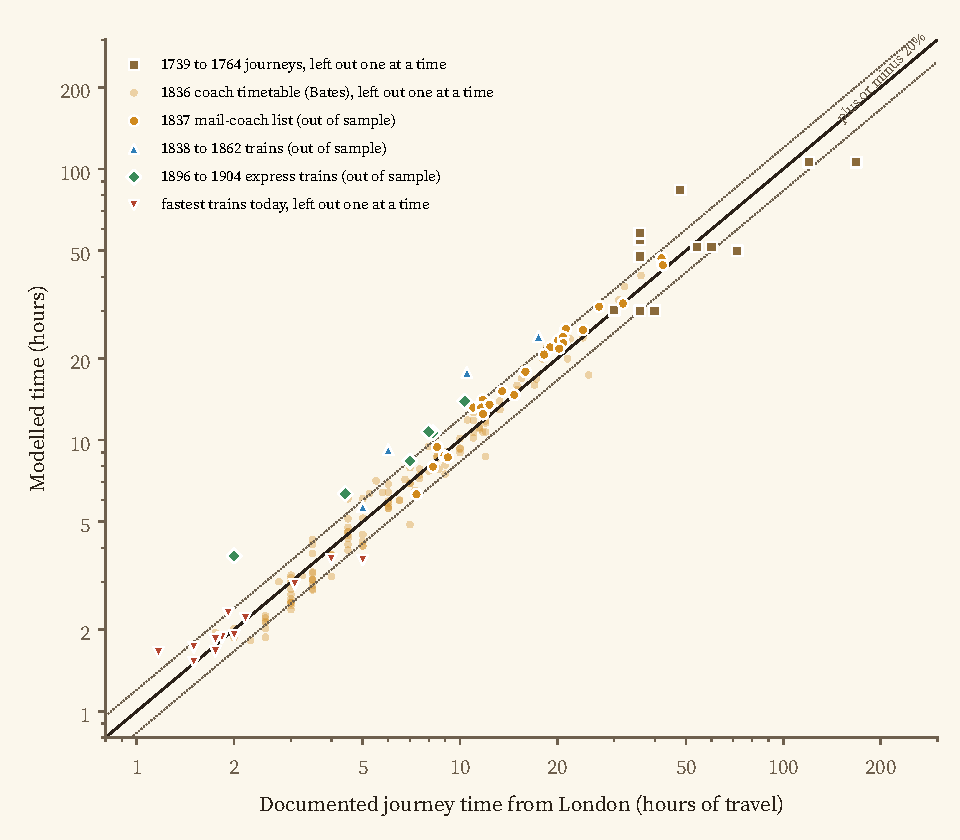
\includegraphics[width=0.7\textwidth]{f_valid.pdf}\caption{Modelled against documented journey times (log scales). Fitted eras are shown leaving each destination out; the 1837 mails, the trains of 1850 and 1910 are out of sample. Dotted lines: within 20\%.}\label{fig:valid}\end{figure}
Table~\ref{tab:valid} and Figure~\ref{fig:valid} compare modelled and documented times. The 1830s model fits the 1836 timetables with a leave-one-out median absolute error of 9.1\% (92\% of termini within 20\%) and almost no bias, and it reproduces the separate 1837 list of mail coaches, which it never saw, with a median error of 11.6\% (96\% within 20\%). The Edinburgh mail of 1837 is modelled at 44.2 hours against 42.4 documented, and the Holyhead mail at 31.1 against 26.9. The largest 1837 errors are Devonport 1837 (+21\%); Bristol 1837 (+20\%); Bath 1837 (+20\%).

The 1750 model is much weaker: its leave-one-out median absolute error is 27.9\% over 12 journeys, above the 25\% that the plan set as evidence against the model. The cited journeys disagree with each other as much as with the model: Edinburgh in ten days (1754) and in a fortnight (1763); Birmingham in three days (1749) and in 40 hours (1740). The largest errors are Newcastle upon Tyne 1764 (+74\%); York 1764 (+61\%); Exeter 1758 (+52\%). By the test set in advance the 1750 model fails, and the 1750 map should be read only as a rough sketch of the order of magnitude, with the uncertainty band in Figure~\ref{fig:maps}.

For the railways, where speeds come from Leunig's averages rather than from the documented times, the model is slower than the famous expresses, as expected: the median absolute error is 46\% for the 4 journeys around 1850 and 34\% for the 6 around 1910, with mean log errors of +0.35 and +0.34. Liverpool in 1851 is modelled at 9.2 hours against six by express \citep{sidney1851}; Edinburgh around 1901 at 10.6 hours against 8.25. Fitting the rail speed to these documented fastest trains instead would give 65 km/h in 1850 and 90 km/h in 1910 on main lines; Section~\ref{sec:robust} reports the maps that result. With only four and six documented journeys these checks are thin, but they all point the same way: the 1850 and 1910 areas in this paper are lower bounds for a traveller who could take the fastest train, not precise estimates. Today's fitted rail model misses the twelve fastest times by a median 5\% when each is left out.

\subsection{A day from London}
\begin{figure}[tbp]\centering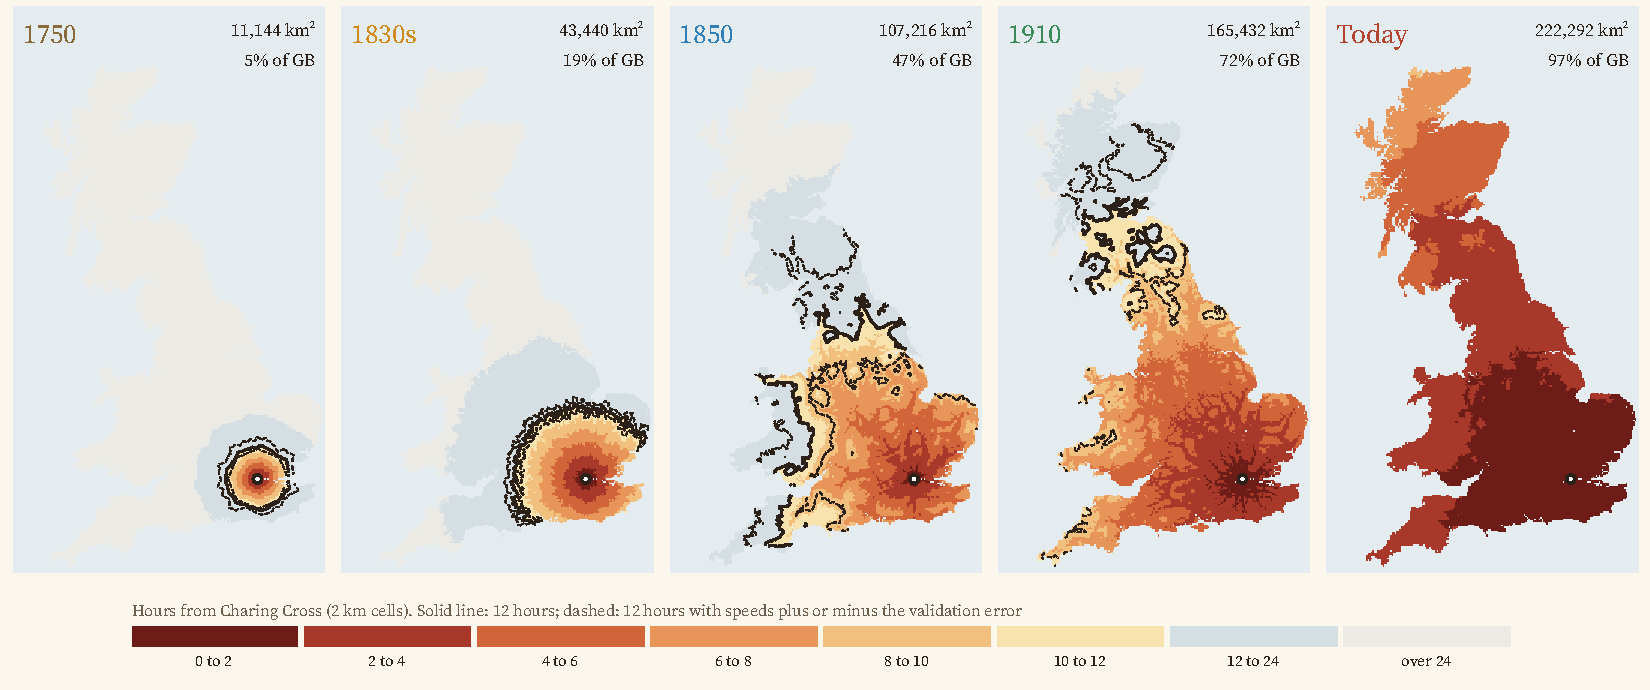
\includegraphics[width=\textwidth]{f_maps.pdf}\caption{Hours of travel from Charing Cross (white dot) in each era, 2 km cells. Solid line: 12 hours; dashed lines: 12 hours with all speeds raised or lowered by the era's median validation error.}\label{fig:maps}\end{figure}
\begin{table}[tbp]\centering\small\caption{Land of Great Britain within 6, 12 and 24 hours of Charing Cross, by era (2 km cells). The range shows the 12-hour area with all speeds lowered and raised by the era's median validation error.}\label{tab:area}\begin{tabular}{lrrrrr}\toprule Era & 6 hours & 12 hours & Share (\%) & Range (\%) & 24 hours\\\midrule
1750 & 2,792 & 11,144 & 4.8 & 4 to 7 & 35,992\\
1830s & 13,496 & 43,440 & 18.9 & 17 to 21 & 105,896\\
1850 & 34,404 & 107,216 & 46.6 & 33 to 61 & 178,276\\
1910 & 89,936 & 165,432 & 71.9 & 62 to 80 & 213,264\\
Today & 205,072 & 222,292 & 96.6 & 97 to 97 & 222,292\\
\bottomrule\end{tabular}\end{table}
\begin{figure}[tbp]\centering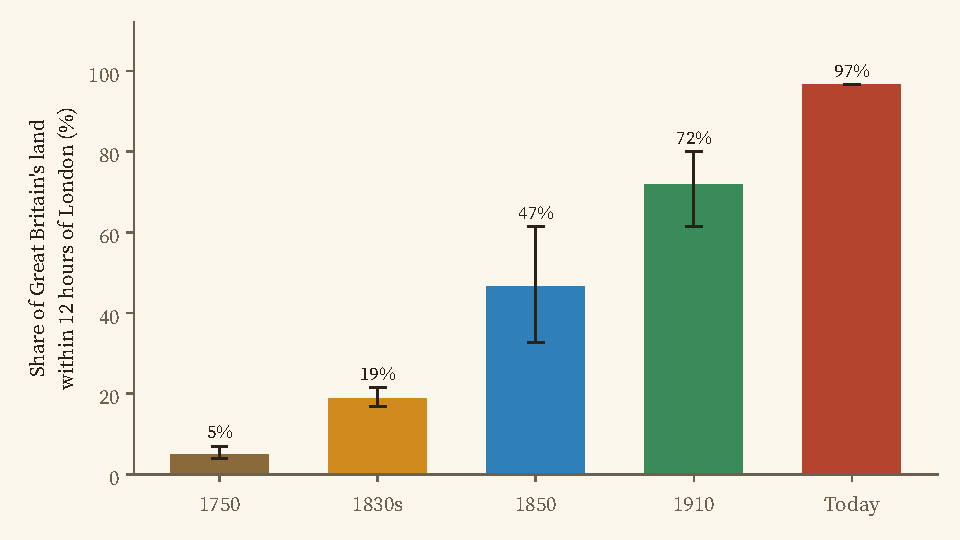
\includegraphics[width=0.7\textwidth]{f_area.pdf}\caption{Share of Great Britain's land within 12 hours of Charing Cross by era; whiskers: speeds lowered and raised by the era's median validation error.}\label{fig:area}\end{figure}
Figure~\ref{fig:maps} shows the five surfaces, Table~\ref{tab:area} the area within six, twelve and 24 hours, and Figure~\ref{fig:area} the share of land within twelve hours. In 1750, a day of coaching from London covered 11,144 km$^2$ (5\% of Great Britain's 230,096 km$^2$ of land in the model), the farthest cell lying 66 km from Charing Cross in a straight line; with speeds raised or lowered by the era's validation error the share is 4 to 7\%. By the 1830s the area within a day had grown to 43,440 km$^2$ (19\%), 3.9 times the 1750 area, reaching 150 km. The railway of 1850 then raised it to 107,216 km$^2$ (47\%), 2.5 times the 1830s area in about fifteen years, the fastest gain per year between any two of the five dates (the 1750 to 1830s gain, 3.9-fold, took more than eighty years). The 1910 network reached 165,432 km$^2$ (72\%) and today 222,292 km$^2$ (97\%), 20 times the area of 1750. Of the 65 towns on the map, 3 were within a day of London in 1750, 14 in the 1830s, 45 in 1850, 57 in 1910 and 63 today.

The shapes differ as much as the areas. The 1750 and 1830s surfaces are close to circular, because the turnpikes radiated from London in every direction and the coach ran at much the same speed on all of them. In 1850 the inner hours follow the main lines out of London like the spokes of a star, and the edge of the day is ragged: it runs out along the trunk lines to Lancashire, Yorkshire and Holyhead (11.2 hours) while parts of Wales and the south-west remain beyond it. In 1910 the denser network fills most of the gaps and the day reaches Edinburgh and Glasgow; today every mainland town on the map is within it (Wick in 7.4 hours), and the land beyond a day lies on islands without a modelled crossing.

\subsection{Towns and the road north}
\begin{table}[tbp]\centering\small\caption{Modelled hours from Charing Cross to selected towns.}\label{tab:towns}\begin{tabular}{lrrrrr}\toprule Town & 1750 & 1830s & 1850 & 1910 & Today\\\midrule
Brighton & 15.7 & 6.4 & 4.0 & 2.0 & 0.9\\
Oxford & 15.9 & 7.1 & 4.7 & 2.6 & 1.0\\
Bristol & 32.6 & 14.2 & 6.4 & 3.6 & 1.4\\
Birmingham & 31.5 & 13.4 & 6.2 & 3.6 & 1.4\\
York & 56.7 & 24.0 & 9.7 & 5.8 & 2.1\\
Manchester & 52.0 & 22.2 & 8.6 & 5.6 & 2.0\\
Exeter & 53.8 & 20.8 & 9.5 & 5.2 & 1.9\\
Holyhead & 75.3 & 31.1 & 11.2 & 7.2 & 2.8\\
Newcastle & 78.7 & 33.4 & 13.6 & 8.4 & 2.7\\
Edinburgh & 108.9 & 44.4 & 17.6 & 10.7 & 3.6\\
Glasgow & 114.2 & 46.9 & 18.0 & 10.9 & 3.6\\
Aberdeen & 145.2 & 58.4 & 24.9 & 14.3 & 4.6\\
Inverness & 149.4 & 62.5 & 33.8 & 16.1 & 5.4\\
Wick & 179.1 & 74.3 & 45.5 & 26.6 & 7.4\\
\bottomrule\end{tabular}\end{table}
\begin{figure}[tbp]\centering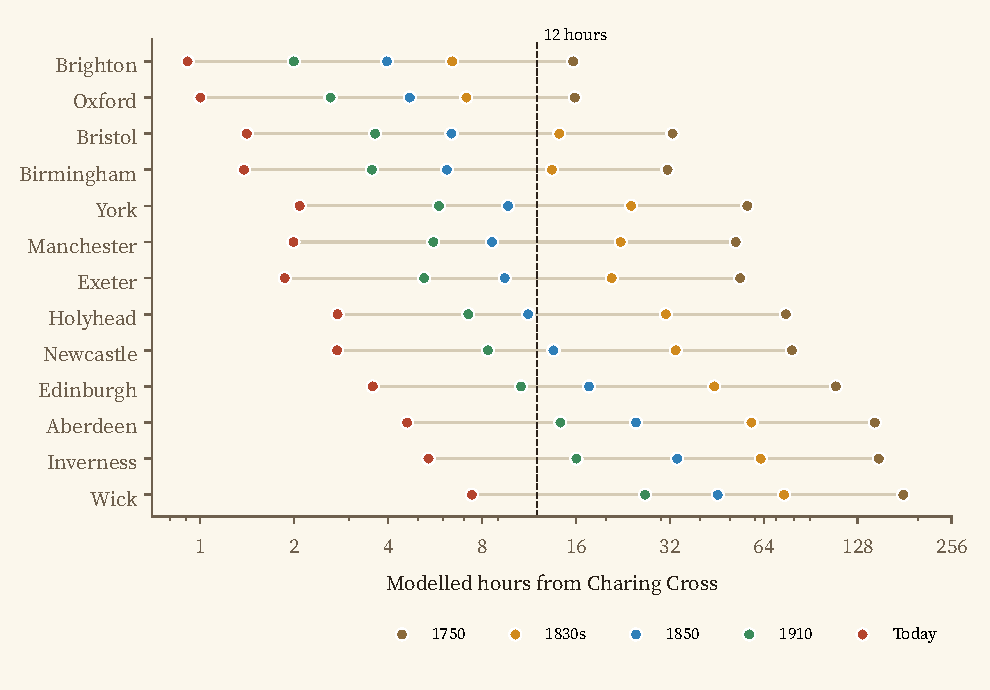
\includegraphics[width=0.75\textwidth]{f_towns.pdf}\caption{Modelled hours from Charing Cross to selected towns by era.}\label{fig:towns}\end{figure}
\begin{figure}[tbp]\centering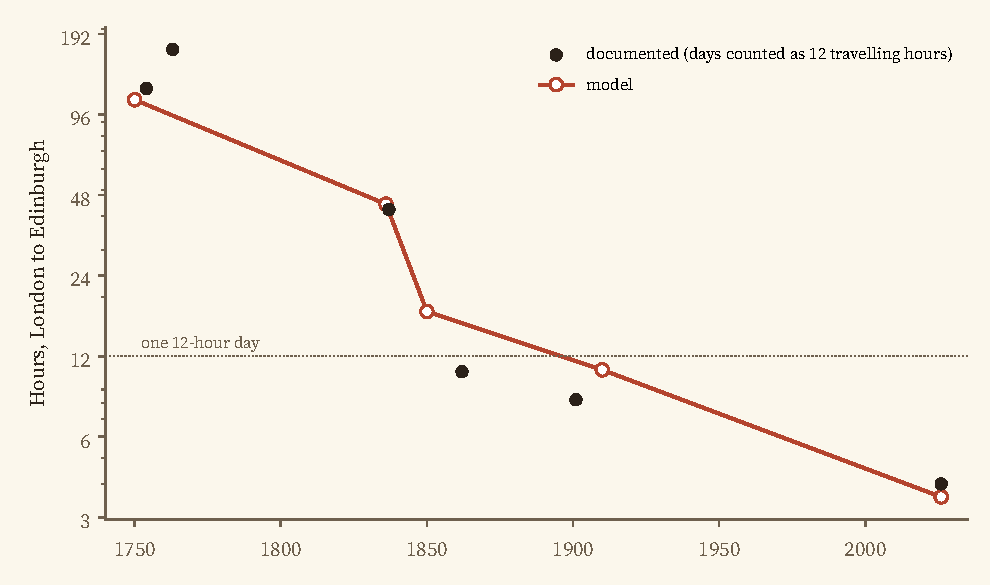
\includegraphics[width=0.75\textwidth]{f_edinburgh.pdf}\caption{London to Edinburgh: documented times (days counted as 12 travelling hours) and the model.}\label{fig:edinburgh}\end{figure}
Table~\ref{tab:towns} gives modelled hours to selected towns and Figure~\ref{fig:towns} plots them. Edinburgh, the classic test of the road north, is 109 hours of travel from London in the 1750 model (9 twelve-hour days), 44 in the 1830s, 17.6 in 1850, 10.7 in 1910 and 3.6 today (Figure~\ref{fig:edinburgh}). In Janelle's terms the model's London to Edinburgh time fell by 45 minutes a year between 1750 and 1836, 115 minutes a year between 1836 and 1850, 7 between 1850 and 1910 and 3.7 since. The fall between 1750 and the 1830s is the largest in absolute terms, because the starting point was so far away; the fall between 1836 and 1850 is the fastest per year. Manchester went from 52 hours to 22, 8.6, 5.6 and 2.0; Bristol from 33 to 14.2, 6.4, 3.6 and 1.4.

\section{Robustness}\label{sec:robust}
\begin{table}[tbp]\centering\small\caption{Sensitivity: share of Great Britain's land within the day (\%), by era. Blank: not applicable to that era.}\label{tab:sens}\begin{tabular}{lrrrrr}\toprule Check & 1750 & 1830s & 1850 & 1910 & Today\\\midrule
Main model & 5 & 19 & 47 & 72 & 97\\\midrule
Other main roads at 0.4 of turnpike speed & 5 & 18 & 46 & 72 & \\
Other main roads at 0.8 & 5 & 19 & 47 & 72 & \\
Other main roads at turnpike speed & 5 & 20 & 47 & 72 & \\
No waits & 5 & 19 & 52 & 74 & 97\\
Waits of 60 minutes & 5 & 19 & 43 & 70 & 97\\
Walking 4 km/h & 4 & 19 & 46 & 71 & \\
Walking 6 km/h & 6 & 19 & 48 & 73 & \\
Branch lines at 0.35 of main &  &  & 45 & 71 & 97\\
Branch lines at 0.7 of main &  &  & 46 & 72 & 97\\
4 km grid & 5 & 18 & 47 & 70 & 96\\
1910 without inferred lines &  &  &  & 70 & \\
Rail speed fitted to fastest trains &  &  & 60 & 82 & \\
8-hour day & 2 & 10 & 27 & 53 & 96\\
16-hour day & 8 & 29 & 61 & 81 & 97\\
1750 with 10-hour coaching days & 6 & & & & \\
1750 with 14-hour coaching days & 4 & & & & \\
\bottomrule\end{tabular}\end{table}
\begin{figure}[tbp]\centering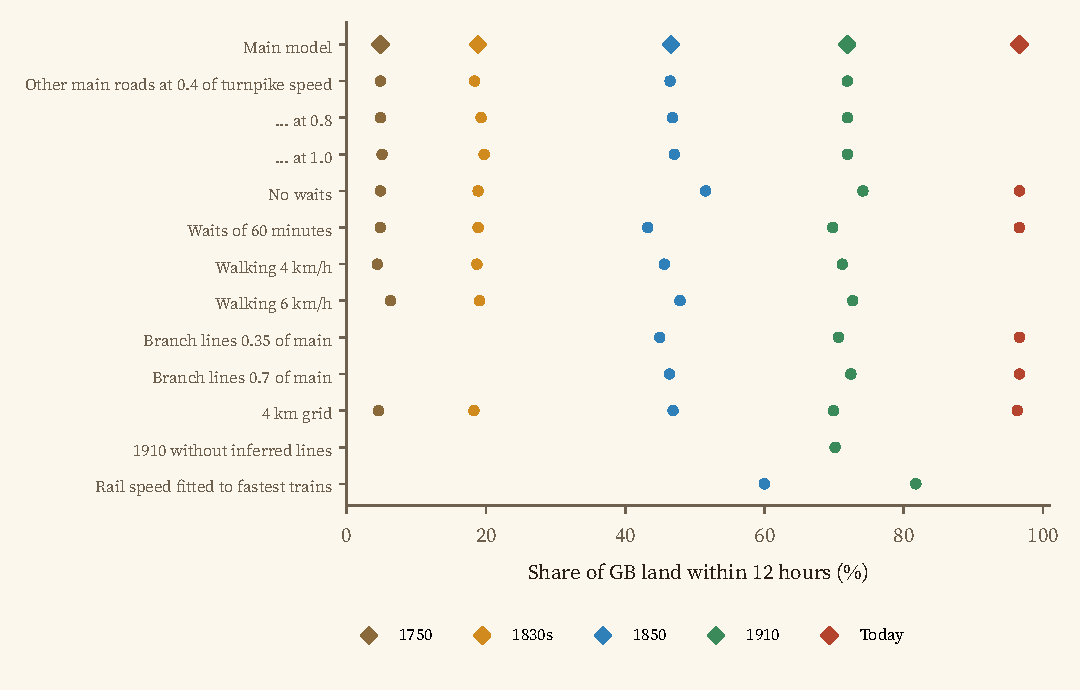
\includegraphics[width=0.8\textwidth]{f_sens.pdf}\caption{Sensitivity of the share of land within 12 hours to the model's assumptions.}\label{fig:sens}\end{figure}
Table~\ref{tab:sens} and Figure~\ref{fig:sens} report the planned checks. Leaving aside the length of the day, the 12-hour share ranges from 4 to 6\% in 1750, 18 to 20\% in the 1830s, 43 to 60\% in 1850, 70 to 82\% in 1910 and 96 to 97\% today. The ordering of the eras never changes. In the coach eras no single assumption moves the share by more than two percentage points; in the railway eras the waits and above all the train speed matter: fitting train speeds to the documented fastest trains rather than Leunig's averages raises the 1850 share to 60\% and the 1910 share to 82\%. Leaving out the inferred lines of 1910 changes the 1910 share to 70\%, so the reconstruction matters mainly for remote branch-line country. A coarser 4 km grid gives nearly the same areas. The length of the day matters most of all: an eight-hour day reaches 2\% of the land in 1750 and 27\% in 1850; a sixteen-hour day 8\% and 61\%.

\section{Discussion}\label{sec:disc}
\subsection{Two waves of convergence}
The five maps show two distinct waves in the shrinking of Britain as seen from London. The first came on the roads. Between 1750 and the 1830s the fitted coach speed on a turnpike rose from 3.6 to 8.4 miles per hour of moving time, and the area within a day grew 3.9-fold. This is consistent with the timing of the gains that \citet{gerhold2014} and \citet{bogart2005} attribute to turnpikes, vehicles and horses, and it is a reminder that the convergence of the coaching age was large in its own right: in the model, the 1830s traveller reached in a day what had taken the 1750 traveller several days. The 1819 fit, at 6.8 mph, sits between the two, as the literature's decade averages would predict.

The second wave came with the railway, and it was faster. Between the 1836 timetables and the 1851 network, about fifteen years, the area within a day grew 2.5-fold, and the shape of the reachable area changed. A coach-era isochrone is a compact, nearly circular patch; the railway isochrone of 1850 is ragged, with its inner hours drawn out along the trunk lines like the spokes of a star, while land between the lines remains far slower to reach. This is what one would expect of a network whose speed lay almost entirely on its links, and it matches the emphasis in the railway literature on the uneven way in which lines and stations reached the population \citep{gregory2010,bogart2022}. Between 1850 and 1910 the gain in area was smaller, 1.5-fold, but the network filled in, and by 1910 almost all of England and Wales, and Edinburgh and Glasgow, were within a day. The twentieth century then added the rest of the mainland, by road as much as by rail. The model's day is a blunt instrument for the period after 1910, because once most of the island is inside the line the area can no longer grow much; the six-hour area in Table~\ref{tab:area} shows that convergence continued long after the twelve-hour area saturated.

\subsection{Why calibrate}
Historical network models usually assume speeds. The exercise here shows why it is worth fitting them where timetables exist and testing them where they do not. With one parameter, the 1830s model reproduces 136 scheduled coach times (median error 9\% leaving each out) and an independent list of 27 mail coaches (median error 12\%), which gives some confidence that the turnpike map, the assumption about non-turnpike roads and the walking links are adequate for the period. The same structure fitted to the much sparser 1750 evidence does not reach the standard set in advance: its leave-one-out median error is 28\%, partly because the cited journeys disagree among themselves, partly because a duration in days does not say how many hours were spent on the road, and partly because the network of 1750 is coded only as turnpike or not, when the condition of an unturnpiked road could range from good to impassable. For the railway eras the comparison with the fastest documented trains exposes a different issue: an average train is not the fastest train. The model is slower than the documented fastest trains by a median 46\% around 1850 and 34\% around 1910, a gap as large as some of the differences between eras. Which is right depends on the question. A traveller who could choose their train, and pay for it, could go further than the maps show; a traveller who took what came would do worse, because the model has no timetable waits beyond its half-hour allowance.

\subsection{Limitations}
Several limitations follow from the data and the design. First, there are no timetables. Coaches and trains are assumed to be available when the traveller arrives, apart from a fixed wait, and connections, night services and Sunday working are ignored. Second, the 1910 network is a reconstruction. Lines that closed after 1910 are inferred as straight links between closed stations; they are shorter than the real lines, may join stations that were never connected, and miss closed lines whose stations were within 2 km of a surviving or 1851 line. Lines opened after 1910 and still open are not removed. The sensitivity check without the inferred lines shows the scale of their effect. Third, the main-line classification for 1850 and 1910 uses today's main lines as a proxy. Fourth, Scotland has no turnpike map, and its main roads are proxied by today's trunk and primary roads; this affects only regions beyond a day from London in the coach eras, but it would matter for a study centred in Scotland. Fifth, the 1750 calibration rests on twelve journeys, several from narrative sources quoting advertisements, which promise rather than record. Sixth, the twelve-hour day is a choice; Table~\ref{tab:sens} shows that an eight or sixteen-hour day changes the areas more than any other assumption, though not their order. Seventh, the model ignores terrain, weather and season, fares and the cost of a horse, and assumes every traveller could ride in a coach or train at all, which in 1750 most people could not afford. Finally, the town list and the origin are fixed: a day from Manchester or Bristol would look different, and the same code could produce it.

\subsection{Future work}
Three sources would remove the largest uncertainties. Leunig's transcriptions of railway timetables for important and minor routes in 1850, 1870, 1887 and 1910, and for 48 routes between 1910 and 2008, are deposited with the UK Data Service and would allow train speeds to be fitted and tested route by route. The full time-dynamic rail lines file would replace the inferred lines of 1910 with the real network. And a systematic collection of dated coach advertisements for the 1740s to 1760s, of the kind Gerhold assembled, would put the 1750 map on the same footing as the 1830s. With timetables, the model could also be extended from a fastest-path model to one that respects departure times, which would bring it closer to what a traveller actually experienced.


\section{Conclusion}\label{sec:conc}
Leaving London at dawn, a traveller of 1750 could reach about 5\% of Great Britain within twelve hours of travel; one of the 1830s, about 19\%; one of 1850, 47\%; of 1910, 72\%; and one today, 97\%. These figures come from a transparent network model built on published historical maps of Britain's roads and railways, with coach speeds fitted to timetables and train speeds taken from published averages, and each era's map has been tested against journeys it did not see. The test is passed comfortably for the 1830s and not passed for 1750, whose map is only a rough sketch. The railway models describe an average train and are slower than the documented expresses by a median 46\% and 34\%, on four and six journeys, so the 1850 and 1910 figures are lower bounds. The ordering of the eras, two waves of convergence, the first on the turnpikes and the second, faster one on the early railways, is unchanged under every assumption varied here. The surfaces, the compiled journey times and the code are released so that others can check them, swap in better data, or ask how far a day reached from somewhere other than London.



\section*{Data availability statement}
Data and code: Zenodo DOI https://doi.org/10.5281/zenodo.24105505. The interactive map is at \url{https://maps.tristanhotham.com/day-from-london/} and the repository at \url{https://github.com/Tristan-Hotham/day-from-london}. The repository holds the derived travel-time grids, isochrones, fitted speeds, the documented journey times with their sources and the model's predictions, and the code. The turnpike road map and the London coach services \citep{rosevear2023tp,rosevear2023coach} were obtained from openICPSR, whose project pages state no licence; they are not redistributed, and only derived results are shared. The 1851 rail lines \citep{satchell2023} are CC BY 4.0; OpenStreetMap data (via OpenFreeMap) are ODbL.

\section*{AI statement}
I wrote the text, with drafting and editing assistance from Claude (Anthropic), which also helped prepare the analysis code. I reviewed and checked all text and results.

\begin{thebibliography}{99}
\bibitem[Albert(1972)]{albert1972} Albert, W. (1972) \textit{The Turnpike Road System in England 1663 to 1840}. Cambridge: Cambridge University Press.
\bibitem[Alvarez-Palau et al.(2017)]{alvarez2017} Alvarez-Palau, E. J., Bogart, D., Dunn, O., Satchell, M. and Shaw-Taylor, L. (2017) Growth before steam: a GIS approach to estimating multi-modal transport costs and productivity growth in England, 1680 to 1830. Working paper, University of California, Irvine. \url{https://sites.socsci.uci.edu/~dbogart/growthbeforesteam_may42017.pdf}.
\bibitem[Axhausen et al.(2011)]{axhausen2011} Axhausen, K. W., Fr\"ohlich, P. and Tschopp, M. (2011) Changes in Swiss accessibility since 1850. \textit{Research in Transportation Economics} 31(1), 72 to 80.
\bibitem[Bates(1969)]{bates1969} Bates, A. (1969) \textit{Directory of Stage Coach Services 1836}. Newton Abbot: David and Charles.
\bibitem[Bogart(2005)]{bogart2005} Bogart, D. (2005) Turnpike trusts and the transportation revolution in 18th century England. \textit{Explorations in Economic History} 42(4), 479 to 508. doi:10.1016/j.eeh.2005.02.001.
\bibitem[Bogart et al.(2022)]{bogart2022} Bogart, D., You, X., Alvarez-Palau, E. J., Satchell, M. and Shaw-Taylor, L. (2022) Railways, divergence, and structural change in 19th century England and Wales. \textit{Journal of Urban Economics} 128, 103390. doi:10.1016/j.jue.2021.103390.
\bibitem[Department for Transport(2025)]{dft2025} Department for Transport (2025) \textit{Vehicle Speed Compliance Statistics for Great Britain: 2024}. London: Department for Transport. \url{https://www.gov.uk/government/statistics/vehicle-speed-compliance-statistics-for-great-britain-2024}.
\bibitem[Dijkstra(1959)]{dijkstra1959} Dijkstra, E. W. (1959) A note on two problems in connexion with graphs. \textit{Numerische Mathematik} 1, 269 to 271. doi:10.1007/BF01386390.
\bibitem[Gerhold(2005)]{gerhold2005} Gerhold, D. (2005) \textit{Carriers and Coachmasters: Trade and Travel before the Turnpikes}. Chichester: Phillimore.
\bibitem[Gerhold(2014)]{gerhold2014} Gerhold, D. (2014) The development of stage coaching and the impact of turnpike roads, 1653 to 1840. \textit{Economic History Review} 67(3), 818 to 845. doi:10.1111/1468-0289.12048.
\bibitem[Great North Road(n.d.)]{gnrsite} Great North Road (n.d.) Stage-coach history. \url{https://greatnorthroad.co.uk/?p=5891} (accessed 2026), citing Gerhold's map of York services in 1764.
\bibitem[Gregory and Mart\'i-Henneberg(2010)]{gregory2010} Gregory, I. N. and Mart\'i-Henneberg, J. (2010) The railways, urbanization, and local demography in England and Wales, 1825 to 1911. \textit{Social Science History} 34(2), 199 to 228. doi:10.1017/S0145553200011214.
\bibitem[Haklay(2010)]{haklay2010} Haklay, M. (2010) How good is volunteered geographical information? A comparative study of OpenStreetMap and Ordnance Survey datasets. \textit{Environment and Planning B: Planning and Design} 37(4), 682 to 703. doi:10.1068/b35097.
\bibitem[Harper(1899)]{harper1899} Harper, C. G. (1899) \textit{The Exeter Road: The Story of the West of England Highway}. London: Chapman and Hall.
\bibitem[Harper(1902)]{harper1902} Harper, C. G. (1902) \textit{The Holyhead Road: The Mail-Coach Road to Dublin}, vol. I. London: Chapman and Hall.
\bibitem[Harper(1903)]{harper1903} Harper, C. G. (1903) \textit{Stage-Coach and Mail in Days of Yore}, vol. II. London: Chapman and Hall.
\bibitem[Harper(1922)]{harper1922} Harper, C. G. (1922) \textit{The Great North Road: The Old Mail Road to Scotland. London to York}, 2nd edn (first published 1901). London: Cecil Palmer.
\bibitem[Jackman(1916)]{jackman1916} Jackman, W. T. (1916) \textit{The Development of Transportation in Modern England}. Cambridge: Cambridge University Press.
\bibitem[Janelle(1968)]{janelle1968} Janelle, D. G. (1968) Central place development in a time-space framework. \textit{The Professional Geographer} 20(1), 5 to 10.
\bibitem[Janelle(1969)]{janelle1969} Janelle, D. G. (1969) Spatial reorganization: a model and concept. \textit{Annals of the Association of American Geographers} 59(2), 348 to 364. doi:10.1111/j.1467-8306.1969.tb00675.x.
\bibitem[Leunig(2006)]{leunig2006} Leunig, T. (2006) Time is money: a re-assessment of the passenger social savings from Victorian British railways. \textit{Journal of Economic History} 66(3), 635 to 673. doi:10.1017/S0022050706000283.
\bibitem[Levinson(2008)]{levinson2008} Levinson, D. (2008) Density and dispersion: the co-development of land use and rail in London. \textit{Journal of Economic Geography} 8(1), 55 to 77. doi:10.1093/jeg/lbm038.
\bibitem[Mart\'i-Henneberg(2013)]{marti2013} Mart\'i-Henneberg, J. (2013) European integration and national models for railway networks (1840 to 2010). \textit{Journal of Transport Geography} 26, 126 to 138. doi:10.1016/j.jtrangeo.2012.09.004.
\bibitem[Mart\'i-Henneberg et al.(2017)]{marti2017} Mart\'i-Henneberg, J., Satchell, M., You, X., Shaw-Taylor, L. and Wrigley, E. A. (2017) England, Wales and Scotland rail lines 1807 to 1994 [GIS shapefile; documentation by M. Satchell]. Cambridge Group for the History of Population and Social Structure. \url{https://www.campop.geog.cam.ac.uk/research/occupations/datasets/catalogues/documentation/engwalesscotlandrail_lines1807to1994.pdf}.
\bibitem[Pawson(1977)]{pawson1977} Pawson, E. (1977) \textit{Transport and Economy: The Turnpike Roads of Eighteenth Century Britain}. London: Academic Press.
\bibitem[Pope(1989)]{pope1989} Pope, R. (ed.) (1989) \textit{Atlas of British Social and Economic History since c.1700}. London: Routledge.
\bibitem[Rosevear et al.(2019)]{rosevear2018} Rosevear, A., Bogart, D. and Shaw-Taylor, L. (2019) The spatial patterns of coaching in England and Wales from 1681 to 1836: a geographic information systems approach. \textit{The Journal of Transport History} 40. doi:10.1177/0022526619875258.
\bibitem[Rosevear et al.(2023a)]{rosevear2023tp} Rosevear, A., Bogart, D., Shaw-Taylor, L. and Satchell, M. (2023a) Turnpike Road map for England and Wales 1700 to 1838 [data set; version V2.1, ``turnpikes and main 2026'' shapefile, documentation dated January 2026]. Ann Arbor, MI: Inter-university Consortium for Political and Social Research [distributor], openICPSR project 195126. doi:10.3886/E195126. No licence is stated on the project page.
\bibitem[Rosevear et al.(2023b)]{rosevear2023coach} Rosevear, A., Bogart, D. and Shaw-Taylor, L. (2023b) Stagecoach services in England and Wales 1819 and 1836 [data set, version V2]. Ann Arbor, MI: Inter-university Consortium for Political and Social Research [distributor], openICPSR project 195128. doi:10.3886/E195128V2. No licence is stated on the project page.
\bibitem[Satchell et al.(2023)]{satchell2023} Satchell, M., Wrigley, E. A., Shaw-Taylor, L. M. W., You, X. and Henneberg, J. (2023) 1851 England, Wales and Scotland rail lines [data collection]. Colchester: UK Data Archive. doi:10.5255/UKDA-SN-852991.
\bibitem[Schivelbusch(1986)]{schivelbusch1986} Schivelbusch, W. (1986) \textit{The Railway Journey: The Industrialization of Time and Space in the 19th Century}. Berkeley: University of California Press.
\bibitem[Sidney(1851)]{sidney1851} Sidney, S. (1851) \textit{Rides on Railways}. London (preface dated August 1851).
\bibitem[Smiles(1867)]{smiles1867} Smiles, S. (1867) \textit{The Life of Thomas Telford, Civil Engineer, with an Introductory History of Roads and Travelling in Great Britain}. London: John Murray.
\bibitem[Spiekermann and Wegener(1994)]{spiekermann1994} Spiekermann, K. and Wegener, M. (1994) The shrinking continent: new time-space maps of Europe. \textit{Environment and Planning B: Planning and Design} 21(6), 653 to 673. doi:10.1068/b210653.
\bibitem[Tring Local History Museum(n.d.)]{tring} Tring Local History Museum (n.d.) The train now departing: operational history of the London and Birmingham Railway. \url{https://tringlocalhistorymuseum.org.uk/morehistory/Railway/c13_operational.htm} (accessed 2026).
\bibitem[Visit London(2026)]{visitlondon} Visit London (2026) Trains to London. \url{https://www.visitlondon.com/traveller-information/travel-to-london/trains-to-london} (accessed 2026).
\bibitem[Wikipedia(2026a)]{wiki_cre} Wikipedia contributors (2026a) Cornish Riviera Express. \url{https://en.wikipedia.org/wiki/Cornish_Riviera_Express} (accessed 2026; CC BY-SA 4.0).
\bibitem[Wikipedia(2026b)]{wiki_cornishman} Wikipedia contributors (2026b) The Cornishman (train). \url{https://en.wikipedia.org/wiki/The_Cornishman_(train)} (accessed 2026; CC BY-SA 4.0).
\bibitem[Wikipedia(2026c)]{wiki_fs} Wikipedia contributors (2026c) Flying Scotsman (railway service). \url{https://en.wikipedia.org/wiki/Flying_Scotsman_(railway_service)} (accessed 2026; CC BY-SA 4.0).
\bibitem[Wikipedia(2026d)]{wiki_race} Wikipedia contributors (2026d) Race to the North. \url{https://en.wikipedia.org/wiki/Race_to_the_North} (accessed 2026; CC BY-SA 4.0).
\end{thebibliography}


\clearpage
\appendix
\section{Appendix}
\subsection{Speeds}
\begin{table}[tbp]\centering\small\caption{The speed model. Fitted: chosen to minimise squared log error against documented times; fixed: assumed or from the cited source.}\label{tab:speeds}\begin{tabular}{p{2.1cm}p{6.6cm}rp{3.8cm}}\toprule Era & Element & km/h & Source\\\midrule
1750 & Coach on a turnpike of 1750 & 5.75 & fitted, 12 journeys\\
 & Other main road; Scotland's main roads & 3.45 & 0.6 of turnpike (assumed)\\
1830s & Coach on a turnpike of 1830; Scotland's main roads & 13.5 & fitted, 1836 timetables\\
 & Other main road & 8.1 & 0.6 of turnpike (assumed)\\
1819 check & Coach on a turnpike of 1820 & 11.0 & fitted, 1819 timetables\\
1850 & Main-line train & 42.1 & \citet{leunig2006} $\times$ circuity 1.15\\
 & Branch-line train & 33.0 & minor/important ratio\\
 & Feeder coach on 1838 roads & 13.5 & 1830s fit\\
1910 & Main-line train & 62.6 & \citet{leunig2006} $\times$ circuity 1.05\\
 & Branch-line train & 34.6 & minor/important ratio\\
 & Feeder coach on 1838 roads & 13.5 & 1830s fit\\
Today & Main-line train; branch & 210; 105 & fitted, 12 times; half\\
 & Motorway, trunk, primary, secondary & 100, 80, 60, 45 & fixed, below \citet{dft2025} free-flow\\
 & Between cells (minor roads) & 30 & fixed\\
All before today & Walking between cells & 4.8 & fixed (3 mph)\\
Rail eras & Wait on boarding a train or feeder coach & 30 min & fixed\\
\bottomrule\end{tabular}\end{table}
\subsection{Documented journeys}
{\scriptsize\setlength{\tabcolsep}{3pt}\begin{longtable}{llrrrrp{5.2cm}}\caption{Documented journeys from London and the model. Model: leave-one-out time for 1750 and today, otherwise the model; days counted as 12 travelling hours.}\label{tab:docs}\\\toprule Era & Destination & Year & Documented & Model (h) & Error (\%) & Source\\\midrule\endfirsthead \toprule Era & Destination & Year & Documented & Model (h) & Error (\%) & Source\\\midrule\endhead
1750 & Birmingham & 1749 & 3 days & 30.0 & $-$17 & Smiles 1867\\
1750 & Birmingham & 1740 & 40.00 h & 30.0 & $-$25 & Bogart 2005\\
1750 & Manchester & 1754 & 4.5 days & 51.5 & $-$5 & Smiles 1867\\
1750 & Manchester & 1760 & 60.00 h & 51.5 & $-$14 & Bogart 2005\\
1750 & Sheffield & 1760 & 3 days & 47.5 & +32 & Smiles 1867\\
1750 & Bath & 1763 & 2.5 days & 30.2 & +1 & Smiles 1867\\
1750 & Edinburgh & 1754 & 10 days & 106.0 & $-$12 & Harper 1901 Great North Road\\
1750 & Edinburgh & 1763 & 14 days & 106.0 & $-$37 & Harper 1901 Great North Road\\
1750 & Exeter & 1758 & 3 days & 54.8 & +52 & Harper 1899 Exeter Road\\
1750 & Chester & 1739 & 6 days & 49.9 & $-$31 & Harper 1902 Holyhead Road\\
1750 & York & 1764 & 3 days & 58.0 & +61 & Gerhold via Great North Road site\\
1750 & Newcastle upon Tyne & 1764 & 4 days & 83.6 & +74 & Gerhold via Great North Road site\\
1830s & Bristol & 1837 & 11.75 h & 14.1 & +20 & Harper 1903 vol 2\\
1830s & Devonport & 1837 & 21.23 h & 25.7 & +21 & Harper 1903 vol 2\\
1830s & Birmingham & 1837 & 11.93 h & 13.2 & +11 & Harper 1903 vol 2\\
1830s & Bath & 1837 & 11.00 h & 13.2 & +20 & Harper 1903 vol 2\\
1830s & Manchester & 1837 & 19.00 h & 22.0 & +16 & Harper 1903 vol 2\\
1830s & Halifax & 1837 & 20.08 h & 23.3 & +16 & Harper 1903 vol 2\\
1830s & Liverpool & 1837 & 20.83 h & 24.0 & +15 & Harper 1903 vol 2\\
1830s & Holyhead & 1837 & 26.92 h & 31.1 & +15 & Harper 1903 vol 2\\
1830s & Norwich & 1837 & 11.63 h & 13.2 & +13 & Harper 1903 vol 2\\
1830s & Exeter & 1837 & 18.20 h & 20.6 & +13 & Harper 1903 vol 2\\
1830s & New Holland & 1837 & 18.20 h & 20.7 & +14 & Harper 1903 vol 2\\
1830s & Leeds & 1837 & 20.87 h & 22.8 & +9 & Harper 1903 vol 2\\
1830s & Glasgow & 1837 & 42.00 h & 46.9 & +12 & Harper 1903 vol 2\\
1830s & Southampton & 1837 & 8.50 h & 9.4 & +11 & Harper 1903 vol 2\\
1830s & Edinburgh & 1837 & 42.38 h & 44.2 & +4 & Harper 1903 vol 2\\
1830s & Chester & 1837 & 20.27 h & 21.7 & +7 & Harper 1903 vol 2\\
1830s & Carmarthen & 1837 & 24.00 h & 25.5 & +6 & Harper 1903 vol 2\\
1830s & Worcester & 1837 & 12.33 h & 13.5 & +10 & Harper 1903 vol 2\\
1830s & Great Yarmouth & 1837 & 13.50 h & 15.2 & +12 & Harper 1903 vol 2\\
1830s & Louth & 1837 & 15.93 h & 17.9 & +12 & Harper 1903 vol 2\\
1830s & Stroud & 1837 & 11.78 h & 12.5 & +6 & Harper 1903 vol 2\\
1830s & Wells & 1837 & 14.72 h & 14.7 & $-$0 & Harper 1903 vol 2\\
1830s & Falmouth & 1837 & 31.92 h & 31.9 & $-$0 & Harper 1903 vol 2\\
1830s & Dover & 1837 & 8.95 h & 8.8 & $-$2 & Harper 1903 vol 2\\
1830s & Hastings & 1837 & 8.25 h & 8.0 & $-$3 & Harper 1903 vol 2\\
1830s & Portsmouth & 1837 & 9.17 h & 8.6 & $-$6 & Harper 1903 vol 2\\
1830s & Brighton & 1837 & 7.33 h & 6.3 & $-$14 & Harper 1903 vol 2\\
1850 & Liverpool & 1851 & 6.00 h & 9.2 & +54 & Sidney 1851\\
1850 & Aberdeen & 1855 & 17.50 h & 24.1 & +38 & Wikipedia Race to the North\\
1850 & Edinburgh & 1862 & 10.50 h & 17.8 & +69 & Wikipedia Flying Scotsman (railway service)\\
1850 & Birmingham & 1838 & 5.00 h & 5.7 & +14 & Tring Local History Museum\\
1910 & Edinburgh & 1901 & 8.25 h & 10.6 & +29 & Wikipedia Flying Scotsman (railway service)\\
1910 & Glasgow & 1903 & 8.00 h & 10.7 & +34 & Harper 1903 vol 2\\
1910 & Plymouth & 1904 & 4.42 h & 6.3 & +44 & Wikipedia Cornish Riviera Express\\
1910 & Penzance & 1904 & 7.00 h & 8.4 & +20 & Wikipedia Cornish Riviera Express\\
1910 & Bristol & 1903 & 2.00 h & 3.7 & +87 & Wikipedia The Cornishman (train)\\
1910 & Aberdeen & 1896 & 10.33 h & 13.9 & +35 & Wikipedia Race to the North\\
Today & Bristol & 2026 & 1.75 h & 1.7 & $-$5 & Visit London\\
Today & Cardiff & 2026 & 1.83 h & 1.9 & +2 & Visit London\\
Today & Birmingham & 2026 & 1.50 h & 1.5 & +1 & Visit London\\
Today & Manchester & 2026 & 2.17 h & 2.2 & +1 & Visit London\\
Today & York & 2026 & 1.92 h & 2.3 & +20 & Visit London\\
Today & Leicester & 2026 & 1.17 h & 1.6 & +41 & Visit London\\
Today & Nottingham & 2026 & 1.75 h & 1.8 & +5 & Visit London\\
Today & Derby & 2026 & 1.50 h & 1.7 & +15 & Visit London\\
Today & Sheffield & 2026 & 2.00 h & 1.9 & $-$5 & Visit London\\
Today & Newcastle upon Tyne & 2026 & 3.08 h & 2.9 & $-$5 & Visit London\\
Today & Edinburgh & 2026 & 4.00 h & 3.6 & $-$9 & Visit London\\
Today & Glasgow & 2026 & 5.00 h & 3.6 & $-$28 & Visit London\\
\bottomrule\end{longtable}}
\subsection{Data construction}
The turnpike map has 23,756 line parts after splitting multi-part features; sections coded 7, 8 or 9 for a decade (not yet made, estate roads) are left out of that decade's network. Scotland's proxy roads are 7,062 OpenStreetMap trunk, primary and motorway lines whose midpoints fall in or within 2 km of Scotland's land cells. The 1910 inferred lines join 2,167 closed stations; their total length is 8,827 km. All networks are resampled every 300 m; vertices of different lines closer than 40 m are joined. The land grid uses the ONS December 2023 local authority boundaries (generalised, clipped to the coastline). Coach termini are the end of each service's mapped route farthest from Charing Cross; services whose terminus is within 15 km of Charing Cross are left out. Point times are the minimum, over all graph nodes within 2.5 km, of the node's time plus the walk from it.

\end{document}
